\documentclass{standalone}
\usepackage[T1]{fontenc}
\usepackage[latin2]{inputenc}
\usepackage[english]{babel}
\usepackage{tikz}
\usepackage{times}
\usetikzlibrary{calc,through,backgrounds,positioning,fit}
\usetikzlibrary{shapes,arrows,shadows,calendar}
 
\begin{document}
 
\centering
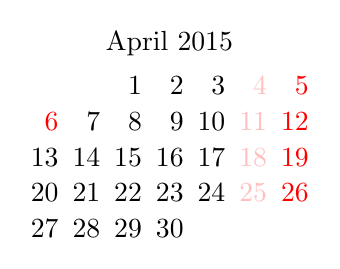
\begin{tikzpicture}[scale=1,inner sep=0.4mm]
\calendar [dates=2015-04-01 to2015-04-last,
week list,
month label above centered,
month text=\%mt \%y-]
if (Sunday) [red]
if (Saturday) [pink]
if (equals=2015-04-06) [red];

\end{tikzpicture}
 
\end{document}